%%%%%%%%%%%%%%%%%%%%%%% file template.tex %%%%%%%%%%%%%%%%%%%%%%%%%
%
% This is a template file for Web of Conferences Journal
%
% Copy it to a new file with a new name and use it as the basis
% for your article
%
%%%%%%%%%%%%%%%%%%%%%%%%%% EDP Science %%%%%%%%%%%%%%%%%%%%%%%%%%%%
%
\documentclass[epj,twocolumn]{webofc}
\usepackage[varg]{txfonts}   % Web of Conferences font
\usepackage{subfig}
\woctitle{Hadron Collider Physics symposium 2012}

%\newcommand{\met}{\mbox{$\raisebox{.3ex}{$\not$}E_T$\hspace*{0.5ex}}} 
\newcommand{\met}{\ensuremath{\rm{E_{T}^{miss}}}}
\newcommand{\lsp}{\ensuremath{\tilde{\chi}_{1}^{0}}}
\newcommand{\chip}{\ensuremath{\tilde{\chi}_{1}^{\pm}}}
\newcommand{\pt}{\ensuremath{p_T}}
\newcommand{\mt}{\ensuremath{M_T}}
\newcommand{\wjets}{\ensuremath{\rm{W+jets}}}
\newcommand{\ttljets}{\ensuremath{t\bar{t}\to\ell+\rm{jets}}}
\newcommand{\ttll}{\ensuremath{t\bar{t}\to\ell\ell}}
\newcommand{\alphat}{\ensuremath{\alpha_{T}}}
%
%
\begin{document}
%
\title{Searches for Top and Bottom Squarks at CMS}
%
% subtitle is optionnal
%
%%%\subtitle{Do you have a subtitle?\\ If so, write it here}

\author{Benjamin Hooberman\inst{1,3}\fnsep\thanks{\email{benhoob@fnal.gov}}
%        Second author\inst{2}\fnsep\thanks{\email{Mail address for second
%             author if necessary}} \and
%        Third author\inst{3}\fnsep\thanks{\email{Mail address for last
%             author if necessary}}
        % etc.
}

\institute{Fermi National Accelerator Laboratory
%\and
%           the second here 
%\and
%           Last address
          }

\abstract{%
  Supersymmetry is a popular extension to the standard problem, which may solve the hierarchy
  problem without fine-tuning if it introduces top and bottom squarks with masses
  not more than several hundred GeV. This note describes three searches for the direct pair production
  of these particles, which are performed
  in the single lepton final state focusing on events with large transverse mass, the same-sign dilepton final state,
  and the all-hadronic final state using the $\alpha_T$ quantity. 
  No evidence for the production of top or bottom squarks is observed.
  The results are used to place stringent constraints on the masses of these particles.
}
%
\maketitle
%

\section{Introduction}
\label{sec:intro}

In this note we describe a search for new physics in the 2011 
opposite sign isolated dilepton sample ($ee$, $e\mu$, and $\mu\mu$).  
The main source of 
isolated dileptons at CMS is Drell Yan and $t\bar{t}$.
Here we concentrate on dileptons with invariant mass inconsistent
with $Z \to ee$ and $Z \to \mu\mu$.  Thus $t\bar{t}$ is the most
important background.  A separate search for new physics in the $Z$ 
sample is described in a separate note\cite{ref:Ztemplates}.
This is an update of an analysis performed on 2010 data~\cite{ref:osnote,ref:ospaper}. 

The search strategy is the following

\begin{itemize}

\item We start out with a pre-selection which is as close as 
possible to the published (or soon to be published) $t\bar{t}$
dilepton analysis\cite{ref:top} (same lepton ID, same jet definitions,
etc.).  We do make a couple of substantive modifications:

\begin{enumerate}
\item The top analysis requires two leptons of $P_T > 20$ GeV.  
 In this
analysis we lower the requirement on the second lepton to $P_T > 10$ 
GeV.  This is motivated by our desire to maintain sensitivity to possible
SUSY signals with relatively low $P_T$ leptons generated in the 
cascade decays of heavy objects.
\item The top analysis requires at least two jets of $P_T > 30$
GeV with \met $>30$ GeV ($ee$ and $e\mu$) or \met $>20$ GeV ($e \mu$).
We tighten the \met cut to 50 GeV and we 
also require that the scalar sum of the $P_T$ of all jets with $P_T > 30$
GeV be $> 100$ GeV.  These requirements considerably
reduce backgrounds to the $t\bar{t}$ sample, {\em e.g.}, backgrounds
from Drell Yan and $W+$jets.
\end{enumerate}

\item The pre-selection consists mostly of $t\bar{t}$ events.  We perform 
data $-$ Monte Carlo comparisons of kinematical distributions.  Assuming
reasonable agreeement for the bulk of $t\bar{t}$ we move on to a 
search for new physics in the tail of the $t\bar{t}$.

\item Our prejudice is that new physics would manifest itself in an
excess of events with high \met and significant hadronic activity.
We define an a-priori search region by tightening the \met and 
hadronic activity requirements such that we expect of order 1\% 
of $t\bar{t}$ events to pass the selection (as predicted by Monte Carlo).

\item We perform a counting experiment in the signal region.  We compare
observed yields with expectations from Monte Carlo and with two independent
data driven techniques (see Section~\ref{sec:abcd} and~\ref{sec:victory}).

\end{itemize}




\section{Search for Top Squark Pair Production in the Single Lepton Final State}
\label{sec:stop}

This section presents the results of a dedicated search for the direct pair production of top squarks, based on an integrated luminosity of 9.7~fb$^{-1}$.
The decay of the top squark depends on the difference between its mass and that of the \lsp\ LSP,
$\Delta m = m_{\tilde{t}}-m_{\lsp}$. If $\Delta m > m_{t}$, the decay $\tilde{t}\to t\lsp$ is expected
to have a large branching fraction. If there is a light chargino \chipm, the decay 
$\tilde{t}\to b\chip\to b W \lsp$ may also be significant.
The pair production of top squarks decaying to either of these channels leads to events with two b-jets, two W bosons,
and two LSPs. Our signal thus resembles SM $t\bar{t}$ production but with larger \met\ from
the invisible LSPs.
We focus here on the single lepton final state, which has a significant branching fraction due to the presence of two W bosons
in the final state,
and smaller SM backgrounds than the all-hadronic final state.
%We thus select events with a single lepton and jets and discriminate between
%signal and background using \met\ and the transverse mass \mt, discussed below.

%\subsection{Event Selection}

We require the presence of exactly one well-identified and isolated electron (e) or muon ($\mu$) with transverse
momentum \pt\ $>$ 30 GeV. 
We select events with at least four jets with \pt\ $>$ 30 GeV,
which must be well-separated from the selected leptons.
At least one of these jets is required to be consistent with coming from the decay of a heavy flavor hadron, as
identified by the Combined Secondary Vertex medium working point (CSVM) b-tagging algorithm~\cite{ref:btag}.
The jet requirements suppress SM backgrounds from W bosons produced in association with jets from initial state
radiation (ISR), referred to as the \wjets\ background. 
The \met\ is required to exceed 50 GeV, suppressing the background from QCD multijet production.

%\subsection{Backgrounds and Estimation Strategy}

The SM background satisfying the above requirements is dominated by $t\bar{t}$ production where
one W boson decays hadronically and the other leptonically (\ttljets), or where both W bosons decay leptonically (\ttll).
There is a small contribution from \wjets, as well as a variety of rare SM
processes, dominated by $t\bar{t}$ produced in association with a vector boson
($t\bar{t}W$ and $t\bar{t}Z$).

To define signal regions, we require the events to have large transverse mass, defined as:

\begin{equation}
M_T = \sqrt{ 2 p_{T}^{\ell} \met ( 1-cos(\Delta\phi))},
\end{equation}

where $p_{T}^{\ell}$ is the lepton transverse momentum and $\Delta\phi$ is the difference in azimuthal angles between the lepton
and \met. This requirement strongly suppresses the background from \ttljets\ and \wjets, which have a kinematic endpoint
at \mt\ $\approx$ $M_W$ since the lepton and neutrino (which produces the \met) are produced together in the decay of the W.
For signal events, as well as for the \ttll\ background, the presence of more than one invisible
particle in the final state leads to events with \mt\ $>>$ $M_W$. 
In addition to the \mt\ requirement, we make several 
\met\ requirements to achieve sensitivity to signals with different mass spectra.
Signal regions with large (small) \met\ requirements are more sensitive to signals with large (small) values of $\Delta m$.

The dominant background in our signal regions is \ttll, which may produce events with large \met\ and \mt\ due to the presence of
more than one invisible neutrino. In order for \ttll\ events to pass the signal region selection, one of the two W leptons must not be identified,
which occurs if it is outside the acceptance, is a hadronic $\tau$ decaying to three charged particles (3-prong decay),
is a hadronic $\tau$ decaying to a single charged particle (1-prong decay), or is an electron or muon that fails the lepton identification
requirements. The latter two categories are suppressed by vetoing events that contain, in addition to the selected lepton, 
a charged particle with \pt\ $>$ 10 GeV that is isolated in space from other energetic charged particles. Furthermore, additional jets 
from initial state or final state radiation (ISR/FSR) are required to satisfy the jet multiplicity requirement $n_{jets}\geq4$. 
To validate and correct the MC modeling of jets from radiation, the MC is compared to data in a dilepton control region dominated by \ttll. 
The MC distribution of $n_{jets}$ is reweighted to match the corresponding data distribution, resulting in small corrections of a few \%.

The SM backgrounds are estimated from events simulated with Monte Carlo (MC) techniques, which are validated and 
(where necessary) corrected using comparisons to data in control regions. The MC expectation is normalized to data in the \mt\ peak region,
in order to remove systematic uncertainties from integrated luminosity and $t\bar{t}$ cross section, and then extrapolated to the 
large \mt\ region. Correction factors and corresponding systematic uncertainties on the MC extrapolation factors are evaluated by 
comparing MC to data in dedicated control regions dominated by \wjets\ (obtained by vetoing events with b-jets), \ttll\ 
(obtained by requiring two selected leptons), and a mixture of \ttll\ and \ttljets\ (obtained by requiring a selected lepton and 
an isolated track). The dominant systematic uncertainty in the background prediction is due to the limited statistical precision in
the data control samples used for these tests.


	\begin{table}[!h]																															
	\begin{center}																															
	{\footnotesize																															
	\begin{tabular}{l||c|c|c|c|c|c|c}																															
	\hline																															
	Sample		&	SRA			&	SRB			&	SRC			&	SRD			&	SRE			&	SRF			&	SRG\\				
	\hline																															
	\hline																															
	\multicolumn{8}{c}{Muon}	\\																														
	\hline																															
	\ttdl\  		&$	330.6	\pm	21.9	$&$	183.4	\pm	20.7	$&$	59.5	\pm	10.0	$&$	22.5	\pm	6.2	$&$	9.0	\pm	3.9	$&$	3.7	\pm	1.8	$&$	2.2	\pm	1.2	$	\\
	\ttsl\ \& single top (1\Lep) 		&$	92.8	\pm	27.5	$&$	41.0	\pm	8.6	$&$	11.5	\pm	3.5	$&$	7.7	\pm	3.4	$&$	0.7	\pm	0.6	$&$	0.3	\pm	0.2	$&$	0.2	\pm	0.2	$	\\
	\wjets\ 		&$	19.2	\pm	4.5	$&$	10.0	\pm	2.2	$&$	3.1	\pm	1.0	$&$	1.2	\pm	0.6	$&$	0.6	\pm	0.4	$&$	0.4	\pm	0.3	$&$	0.2	\pm	0.2	$	\\
	Rare 		&$	33.2	\pm	16.6	$&$	22.7	\pm	11.4	$&$	9.0	\pm	4.5	$&$	4.8	\pm	2.4	$&$	2.9	\pm	1.5	$&$	1.2	\pm	0.6	$&$	1.0	\pm	0.5	$	\\
	\hline																															
	Total 		&$	475.8	\pm	37.8	$&$	257.2	\pm	24.2	$&$	83.2	\pm	11.3	$&$	36.2	\pm	7.4	$&$	13.3	\pm	4.2	$&$	5.5	\pm	1.9	$&$	3.6	\pm	1.3	$	\\
	\hline																															
	\hline																															
	Data 		&$	?			$&$	?			$&$	?			$&$	?			$&$	?			$&$	?			$&$	?			$	\\
	\hline																															
	\hline																															
	\hline																															
	\multicolumn{8}{c}{Electron}	\\																														
	\hline																															
	\ttdl\  		&$	248.1	\pm	16.9	$&$	144.4	\pm	16.6	$&$	51.1	\pm	8.8	$&$	16.2	\pm	4.6	$&$	5.5	\pm	2.5	$&$	2.5	\pm	1.3	$&$	1.3	\pm	0.7	$	\\
	\ttsl\ \& single top (1\Lep) 		&$	68.0	\pm	20.2	$&$	31.2	\pm	6.6	$&$	9.3	\pm	2.8	$&$	4.9	\pm	2.1	$&$	0.5	\pm	0.4	$&$	0.2	\pm	0.2	$&$	0.2	\pm	0.2	$	\\
	\wjets\ 		&$	14.3	\pm	3.3	$&$	7.5	\pm	1.7	$&$	2.4	\pm	0.8	$&$	0.8	\pm	0.4	$&$	0.4	\pm	0.3	$&$	0.3	\pm	0.2	$&$	0.1	\pm	0.2	$	\\
	Rare 		&$	25.8	\pm	12.9	$&$	15.8	\pm	7.9	$&$	7.1	\pm	3.6	$&$	2.9	\pm	1.5	$&$	0.7	\pm	0.4	$&$	0.3	\pm	0.2	$&$	0.1	\pm	0.1	$	\\
	\hline																															
	Total 		&$	356.2	\pm	28.4	$&$	198.9	\pm	19.0	$&$	69.9	\pm	9.7	$&$	24.7	\pm	5.3	$&$	7.1	\pm	2.5	$&$	3.4	\pm	1.3	$&$	1.7	\pm	0.8	$	\\
	\hline																															
	\hline																															
	Data 		&$	?			$&$	?			$&$	?			$&$	?			$&$	?			$&$	?			$&$	?			$	\\
	\hline																															
	\hline																															
	\hline																															
	\multicolumn{8}{c}{Muon+Electron Combined}		\\																													
	\hline																															
	\ttdl\  		&$	578.7	\pm	38.1	$&$	327.8	\pm	36.6	$&$	110.6	\pm	18.3	$&$	38.7	\pm	10.5	$&$	14.5	\pm	6.2	$&$	6.2	\pm	2.9	$&$	3.5	\pm	1.8	$	\\
	\ttsl\ \& single top (1\Lep) 		&$	160.8	\pm	47.7	$&$	72.2	\pm	15.1	$&$	20.8	\pm	6.3	$&$	12.6	\pm	5.4	$&$	1.2	\pm	0.9	$&$	0.6	\pm	0.4	$&$	0.4	\pm	0.3	$	\\
	\wjets\ 		&$	33.5	\pm	8.0	$&$	17.5	\pm	4.1	$&$	5.5	\pm	1.9	$&$	2.0	\pm	1.2	$&$	1.0	\pm	0.7	$&$	0.7	\pm	0.5	$&$	0.3	\pm	0.4	$	\\
	Rare 		&$	59.0	\pm	29.5	$&$	38.5	\pm	19.3	$&$	16.1	\pm	8.1	$&$	7.7	\pm	3.9	$&$	3.6	\pm	1.8	$&$	1.5	\pm	0.8	$&$	1.1	\pm	0.6	$	\\
	\hline																															
	Total 		&$	832.0	\pm	65.7	$&$	456.1	\pm	42.5	$&$	153.0	\pm	20.6	$&$	60.9	\pm	12.4	$&$	20.3	\pm	6.5	$&$	8.9	\pm	3.0	$&$	5.3	\pm	1.9	$	\\
	\hline																															
	\hline																															
	Data 		&$	?			$&$	?			$&$	?			$&$	?			$&$	?			$&$	?			$&$	?			$	\\
	\hline																															
	\end{tabular}}																															
	\caption{The result of the search.																															
	\label{tab:result}																															
	\end{center}}																															
	\end{table}																															


%\subsection{Results}

The results of the search are summarized in Table~\ref{tab:stop}, which displays the SM background expectations and the observed data yields
in the signal regions. The distribution of \met\ after the requirement \mt\ $>$ 120 GeV is displayed in Fig.~\ref{fig:stop}. 
Good agreement between the data and the expected background is observed. We find no evidence
for the pair production of top squarks.

\begin{figure}
% Use the relevant command for your figure-insertion program
% to insert the figure file.
\centering
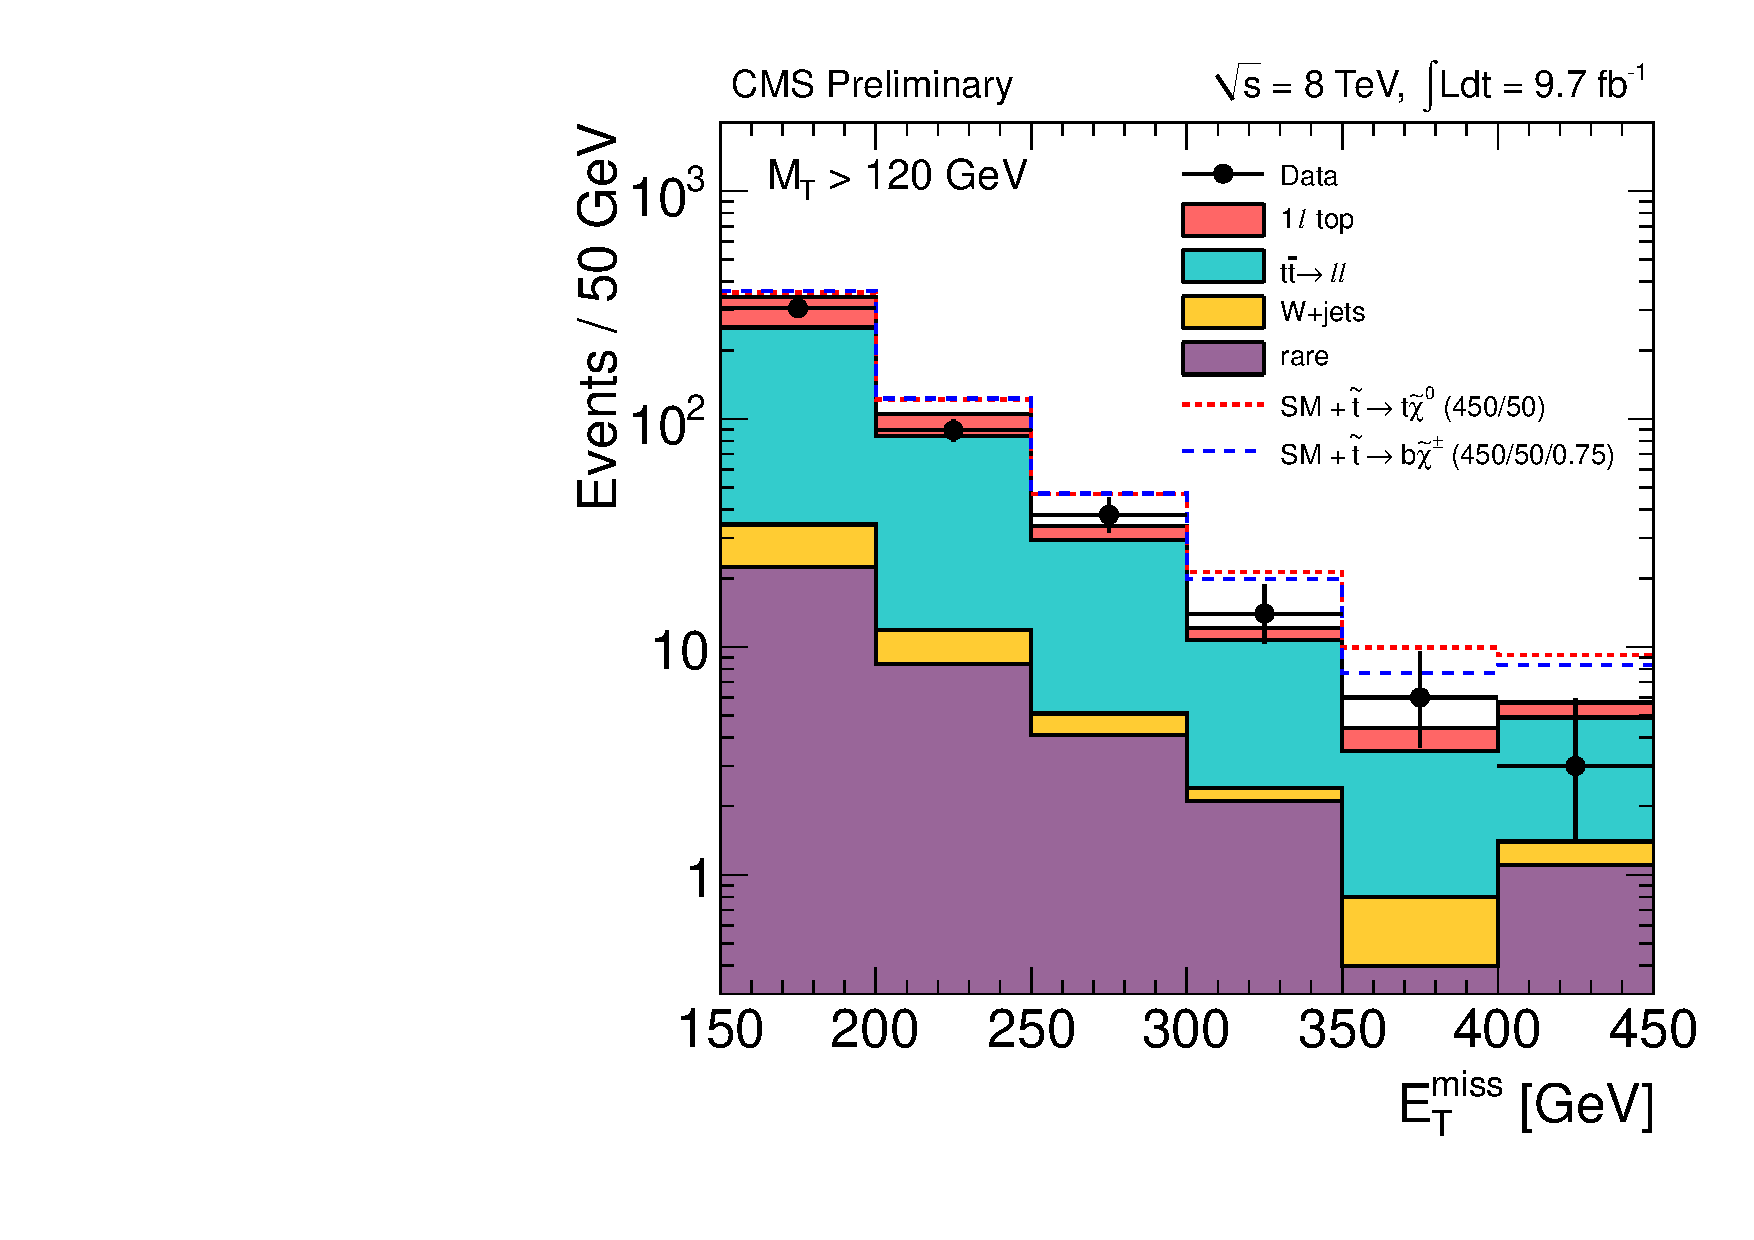
\includegraphics[width=0.4\textwidth]{HCPPlots/stopmet.pdf}
%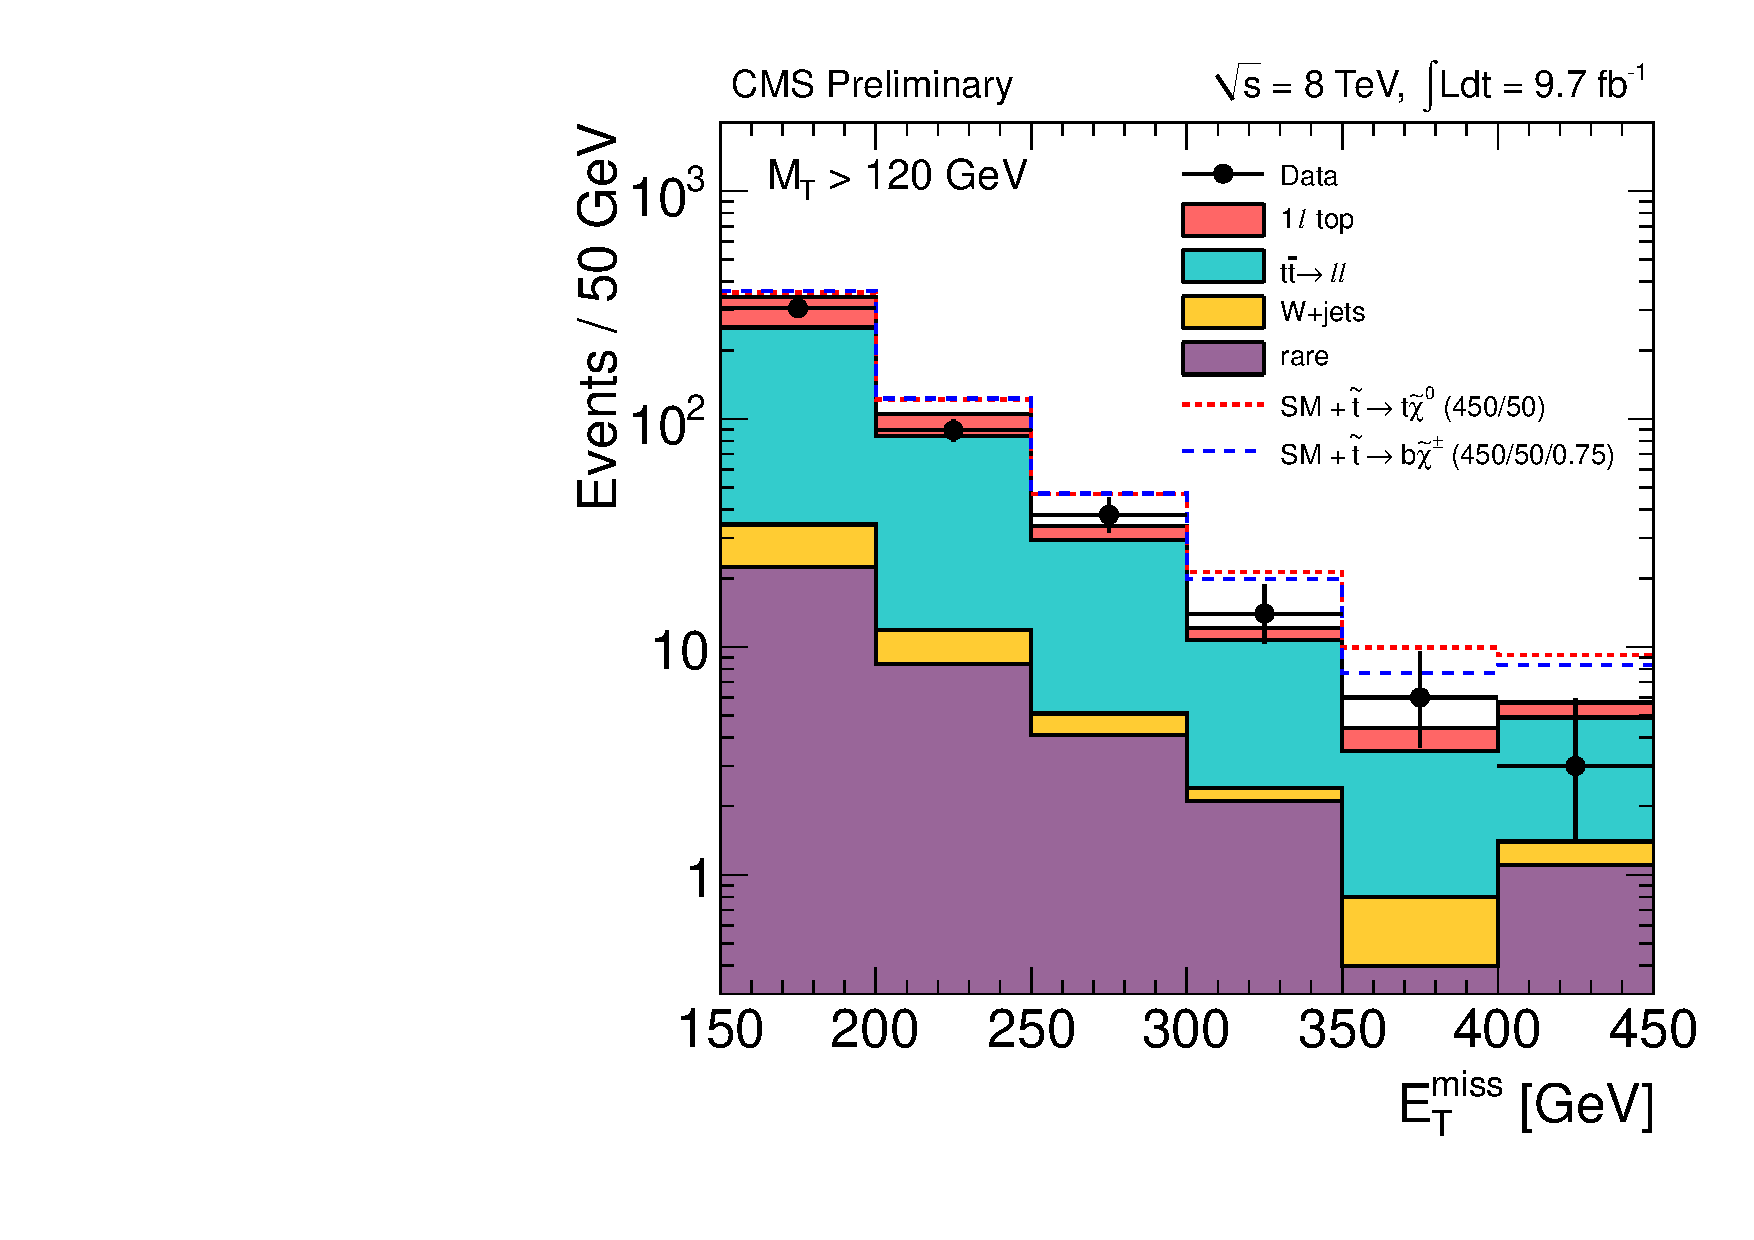
\includegraphics[width=7cm,clip]{HCPPlots/stopmet.pdf}
\caption{The \met\ distribution in data, compared to the sum of expected backgrounds, for the top squark pair search.
Two example signal models with $m_{\tilde{t}}=450$ GeV and $m_{\lsp}=50$ GeV are also indicated. For the $\tilde{t}\to b\chip$
decay, the chargino mass is set by $m_{\chipm}=0.75~m_{\tilde{t}}+0.25~m_{\lsp}$.}
\label{fig:stop}       % Give a unique label
\end{figure}

%\subsection{Interpretation}

%To interpret the results of our search, we consider two signal scenarios of top squark pair production, followed by the decays
%$\tilde{t}\to t\lsp$ and $\tilde{t}\to b\chip\to b W \lsp$. In the first scenario, the only SUSY particles which participate
%are the top squark and \lsp, and the model can thus be parameterized by the masses of these two particles. In the second case
%the chargino mass is also relevant, and we introduce a third parameter $x$, defined as $m_{\chip} = x m_{\lsp} + (1-x) m_{\tilde{t}}$.
%We consider $x=0.5$ and $x=0.75$ (we do not have sensitivity to the $x=0.25$ scenario).

To interpret the results of our search, we consider top squark pair production where both top squarks decay according to 
$\tilde{t}\to t\lsp$, in Fig.~\ref{fig:stop_interpretation}.
The model is parameterized by the masses of the top squark and \lsp. We place upper limits on the signal
production cross section using, for each model point in the 2-dimensional parameter space, the signal region with the best expected
sensitivity. A region of the parameter space is excluded by comparing these cross section upper limits with the theoretical predictions 
for the signal cross section.
%, computed at next-to-leading order including the resummation of soft gluon emission at 
%next-to-leading-logarithmic
%accuracy (NLO+NLL)~\cite{ref:nlonll}. 
Our results probe top squarks with masses up to 430 GeV. For comparison, the requirement that SUSY
provides a natural solution to the hierarchy problem favors top squarks with masses not exceeding 500--700 GeV~\cite{ref:naturalsusy}.
We also interpret our results in the $\tilde{t}\to b\chip\to b W \lsp$ scenario
depicted in Fig.~\ref{fig:diagrams}(b), probing top squarks with masses up to 420 GeV~\cite{ref:stop}.

%The ATLAS experiment has presented a similar search for top squark pairs~\cite{ref:atlasstop}.
%The constraints from ATLAS on the top squark mass are more stringent than those presented here. The ATLAS model assumes large 
%right-handed top quark polarization, while we take the top quark in the $\tilde{t}\to t\lsp$ decay to be unpolarized, 
%resulting in a lower signal selection efficiency in our analysis.

\begin{figure}
% Use the relevant command for your figure-insertion program
% to insert the figure file.
\centering
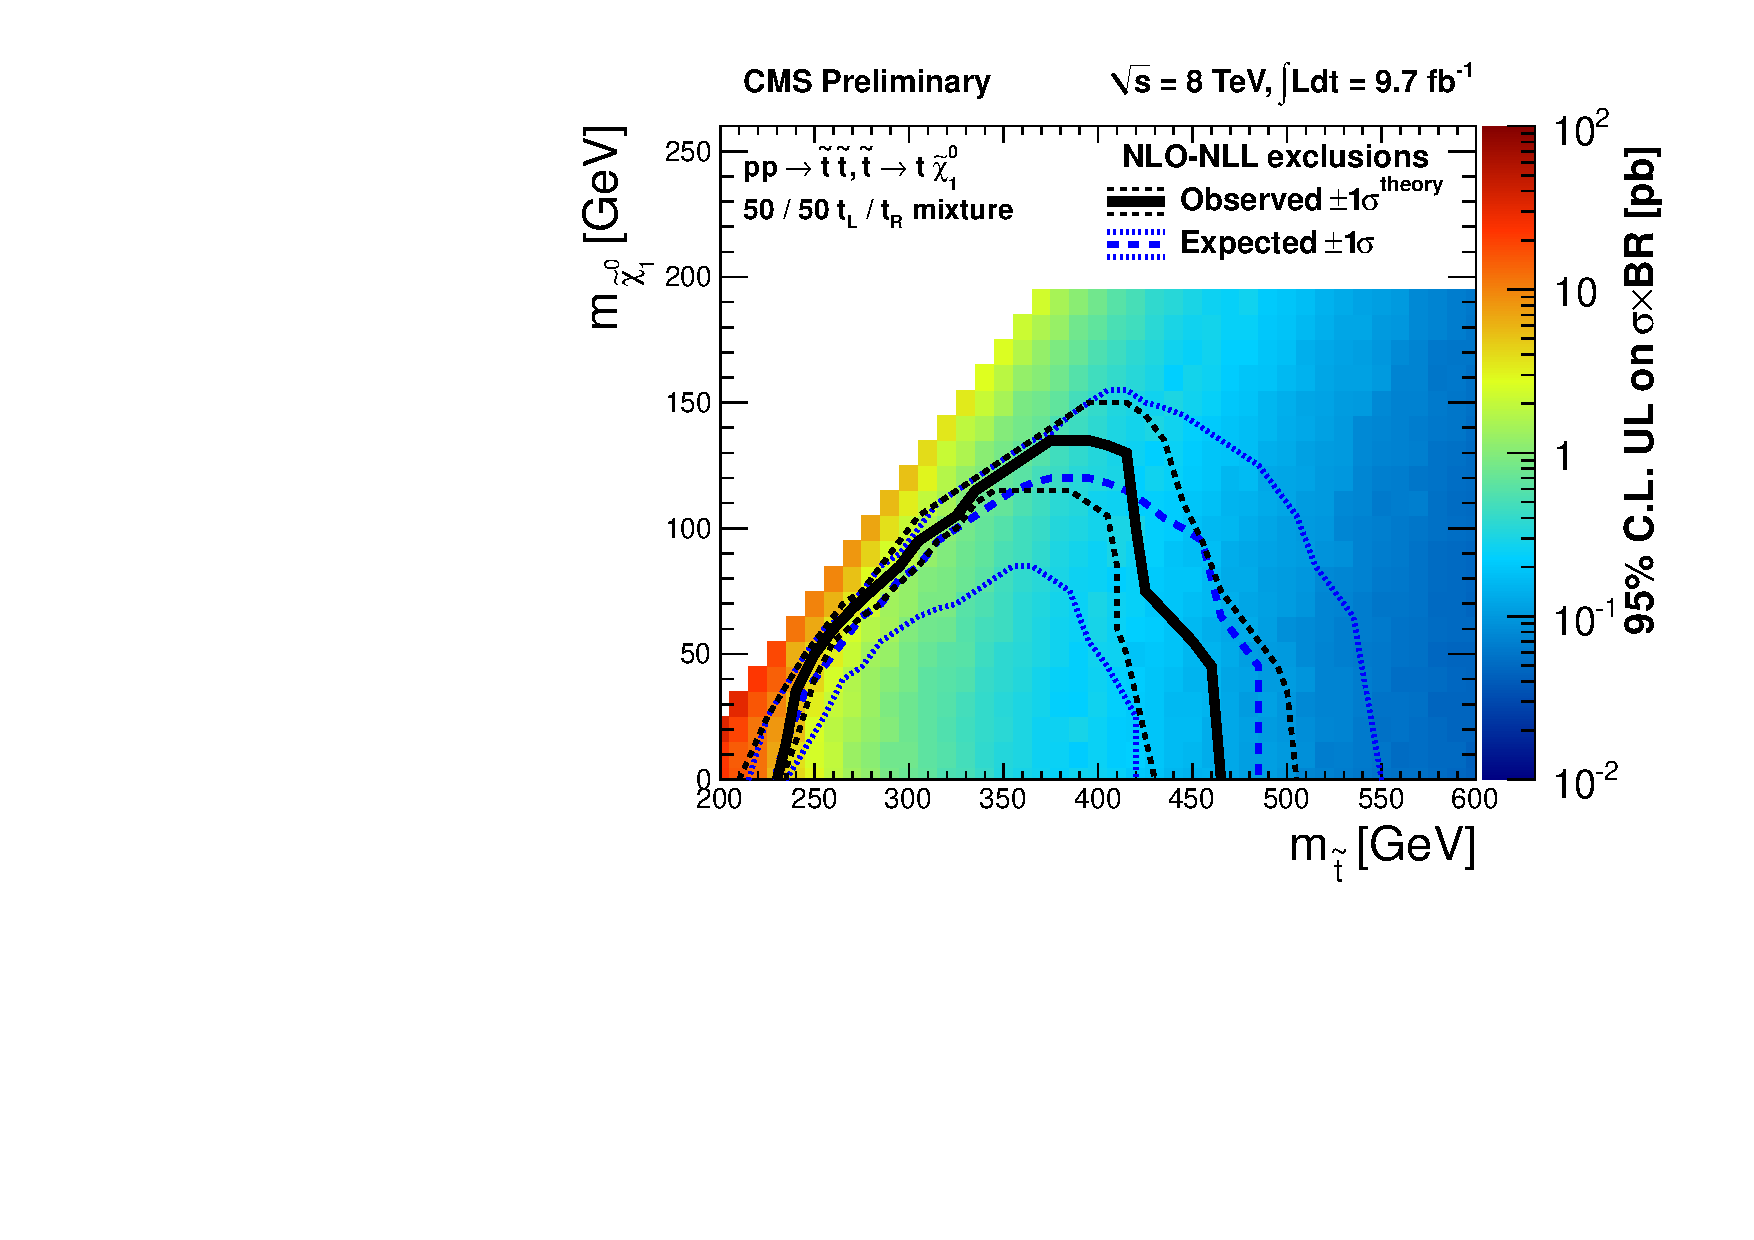
\includegraphics[width=0.5\textwidth]{HCPPlots/stop_interpretation.pdf}
%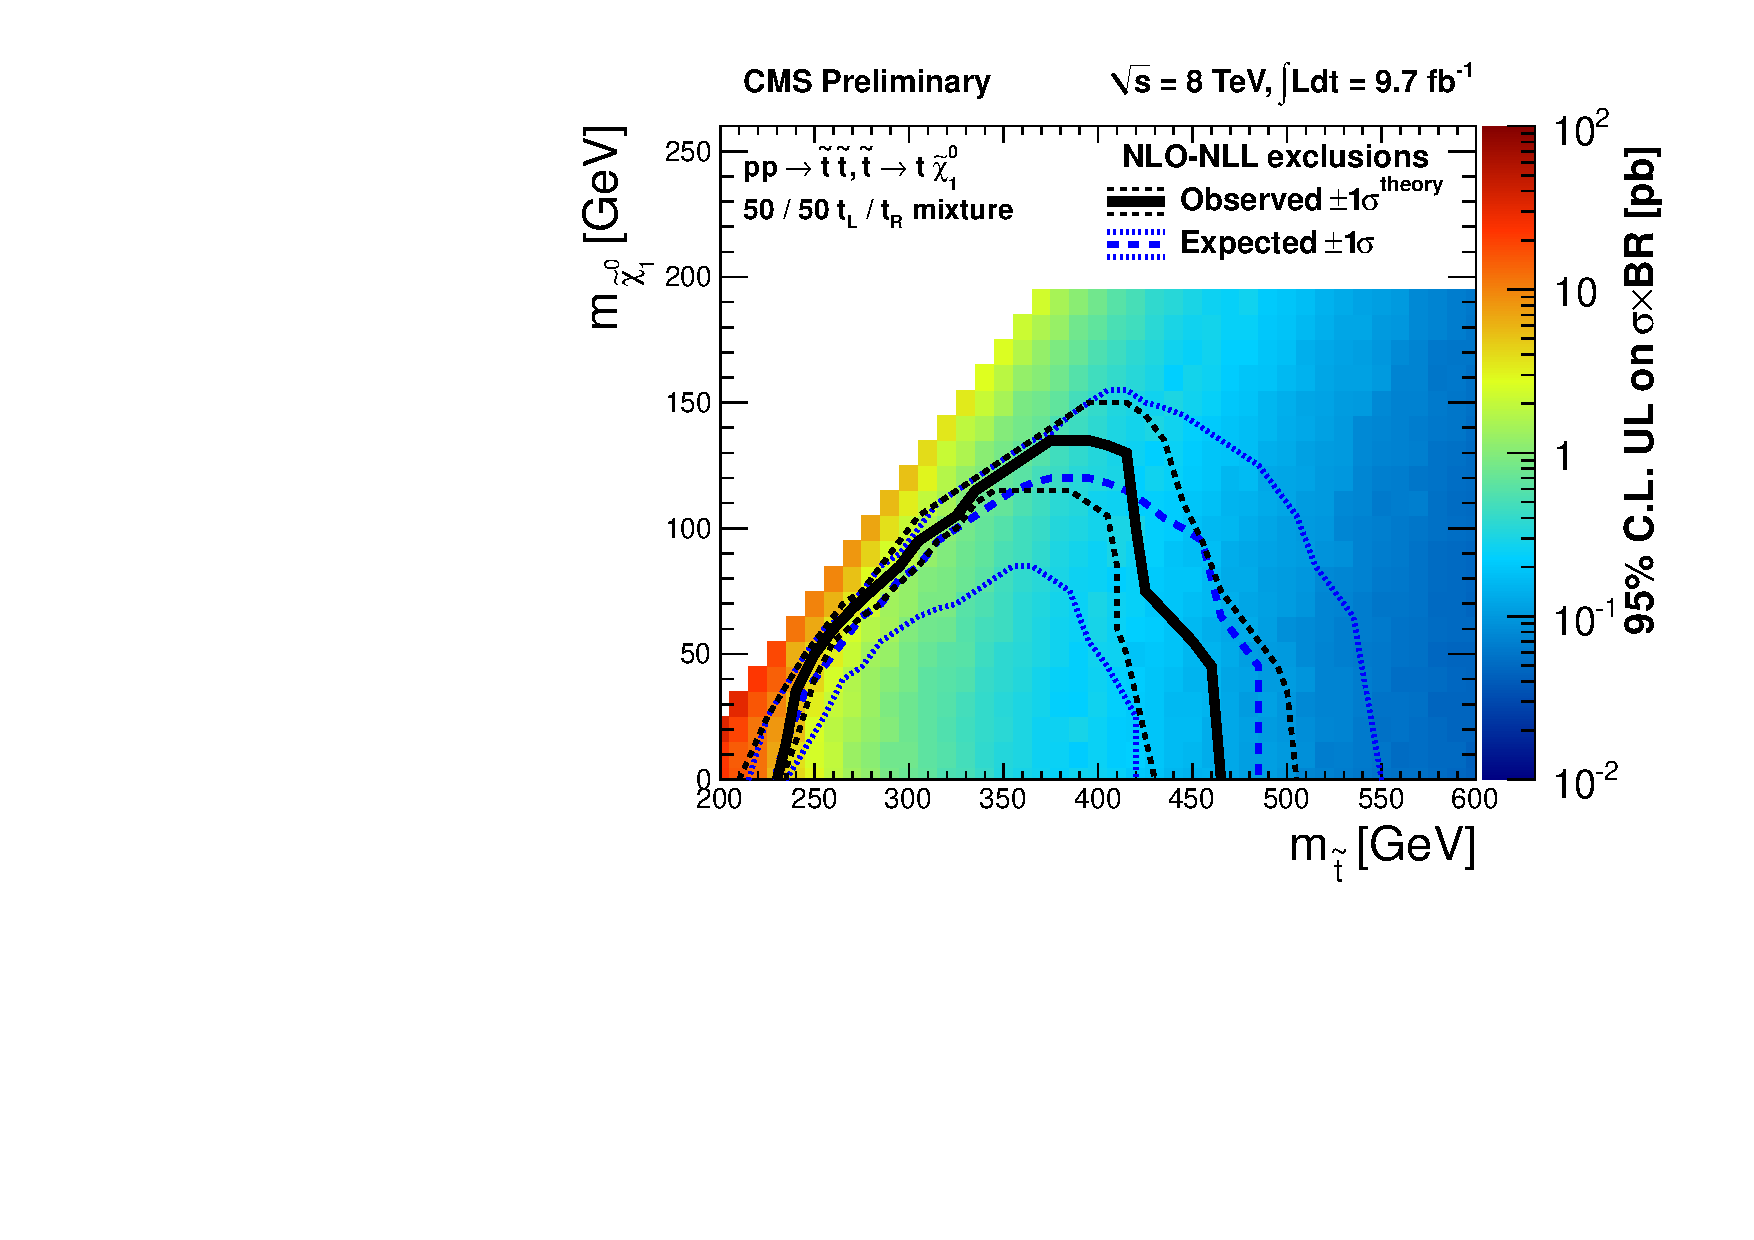
\includegraphics[width=7cm,clip]{HCPPlots/stop_interpretation.pdf}
\caption{Interpretation of the results of the top squark pair search in the $\tilde{t}\to t\lsp$ scenario of 
Fig.~\ref{fig:diagrams}(a). The color scale indicates the cross section upper limits at 95\% confidence level. The solid black contour 
and dashed black contours indicate the observed excluded region and variation in this
excluded region due to the $\pm1\sigma$ uncertainties in the theoretical prediction of the signal cross section. The dashed blue
and dotted blue contours indicate the median and $\pm1\sigma$ expected excluded regions. }
\label{fig:stop_interpretation}       % Give a unique label
\end{figure}

\section{Search in the Same-sign Dilepton Final State}
\label{sec:ss}

A wide variety of new physics processes may produce events with two same-sign (SS) leptons, which provides a very clean
final state due to low SM background expectations. In particular, this final state is sensitive to top
squarks produced in the decays of gluinos (Fig.~\ref{fig:diagrams}X) and to the pair production of bottom squarks
followed by the decay $\tilde{b}\to t \chi^{\pm}$. 

We select events with two leptons (e or $\mu$) with \pt\ $>$ 20 GeV and dilepton invariant mass $m_{\ell\ell}>8$ GeV. 
We reject events with a third lepton with \pt\ $>$ 10 GeV that forms an opposite-sign
same-flavor pair with $76 < m_{\ell\ell} < 106$ GeV with either selected lepton, to suppress
the background from WZ and ZZ. We require the presence of at least two jets with \pt\ $>$ 40 GeV.

This analysis is an extension of a previous search in the same-sign dilepton final state~\cite{ref:ss_inclusive}.
In that analysis, the background is dominated by \ttljets\ where one lepton is from the W decay and the other
lepton is produced in the decay of one of the b-jets. In this analysis we require the presence of at least two
b-tagged jets. The requirement that both b-jets are identified and well separated from the selected leptons
reduces the \ttljets\ background by an order of magnitude. 

There are three sources of SM background. 
The first background source is referred to as ``fake leptons'' and includes leptons from heavy-flavor decay, misidentified hadrons, 
muons from meson decay in flight, or electrons from unidentified photon conversions. 
This background is estimated from a sample of events with at least one lepton that passes a loose selection but fails the full analysis
identification and isolation requirements, using the probability for a fake lepton satisfying the loose selection to also pass the analysis
selection, which is determined based on studies of fake leptons in jet events.
The second background, estimated from MC, consists of rare SM processes and is dominated by $t\bar{t}$W and $t\bar{t}$Z.
The systematic uncertainty on both the fake lepton and rare backgrounds is 50\%. 
A third, small background contributions is from ``charge flips'' and consists of events with opposite-sign leptons where one of the leptons
is an electron whose charge is misreconstructed. This background is based on the MC prediction, which is validated using a sample of Z$\to e^+e^-$ events.

Signal regions are defined by placing additional requirements on the jet multiplicity, b-tagged jet multiplicity, \met, and $H_T$, defined as the scalar 
sum of the transverse momenta of selected jets. The observed data yields in these signal regions is compared to the SM background expectations in 
Table~\ref{tab:ss}. Good agreement is observed between the data and the expected background in all signal regions.

The results are interpreted in the context of the model of gluino-mediated top squark production and bottom squark production indicated in 
Fig.~\ref{fig:diagrams}b and Fig.~\ref{fig:diagrams}d, respectively, in Fig.~\ref{fig:ss_interpretation}. 
For both of these models, the most sensitive signal region is SR6 (see Table~\ref{tab:ss}).
Results are presented in the plane
of squark mass vs. gluino mass, for a fixed choice of \lsp\ and \chip\ masses, and represent lower limits on the gluino mass of approximately 1 TeV in these scenarios.
Additional interpretations for other models and for different choices of \lsp\ and \chip\ masses are presented in Ref.~\cite{ref:ss}.

\begin{figure*}
\centering
%\begin{center}
\begin{tabular}{cc}
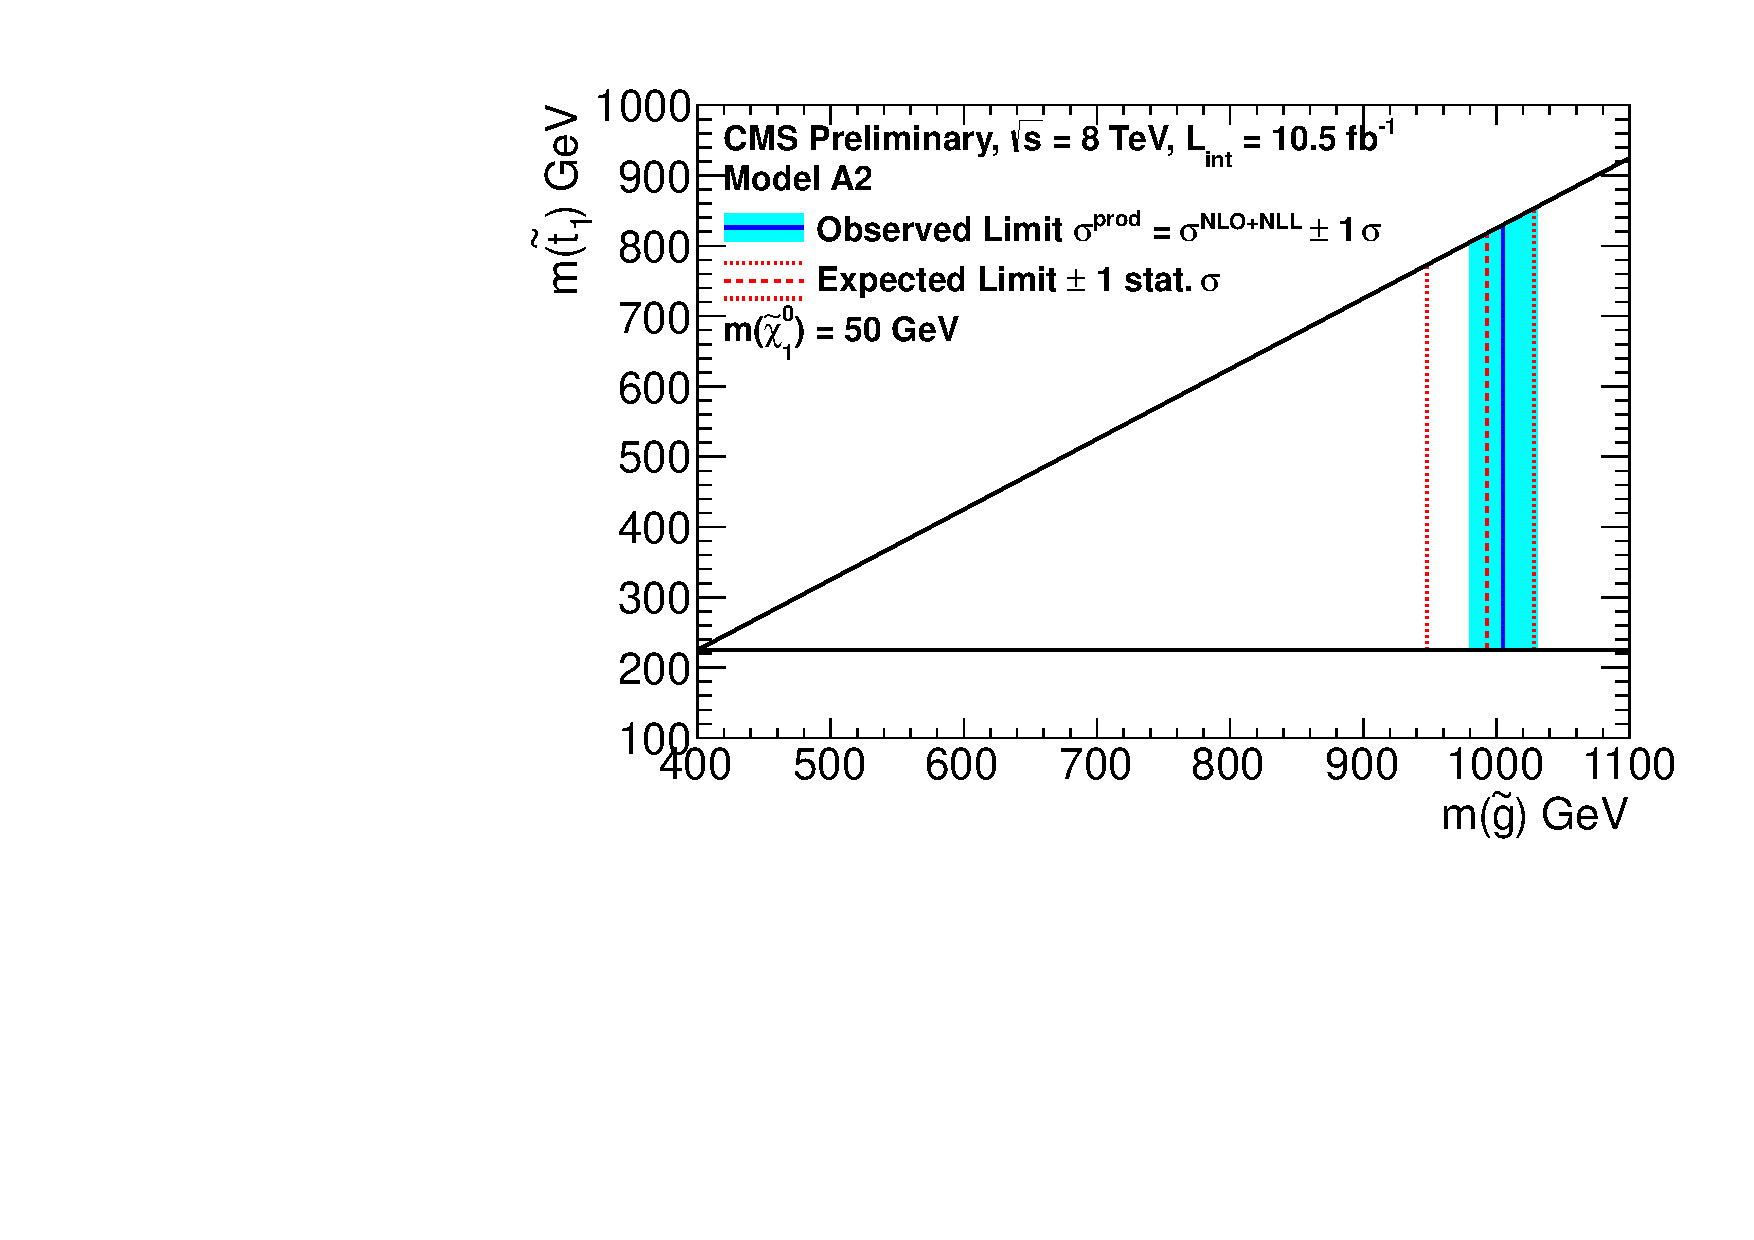
\includegraphics[width=0.45\textwidth]{HCPPlots/SS_A2.pdf} &
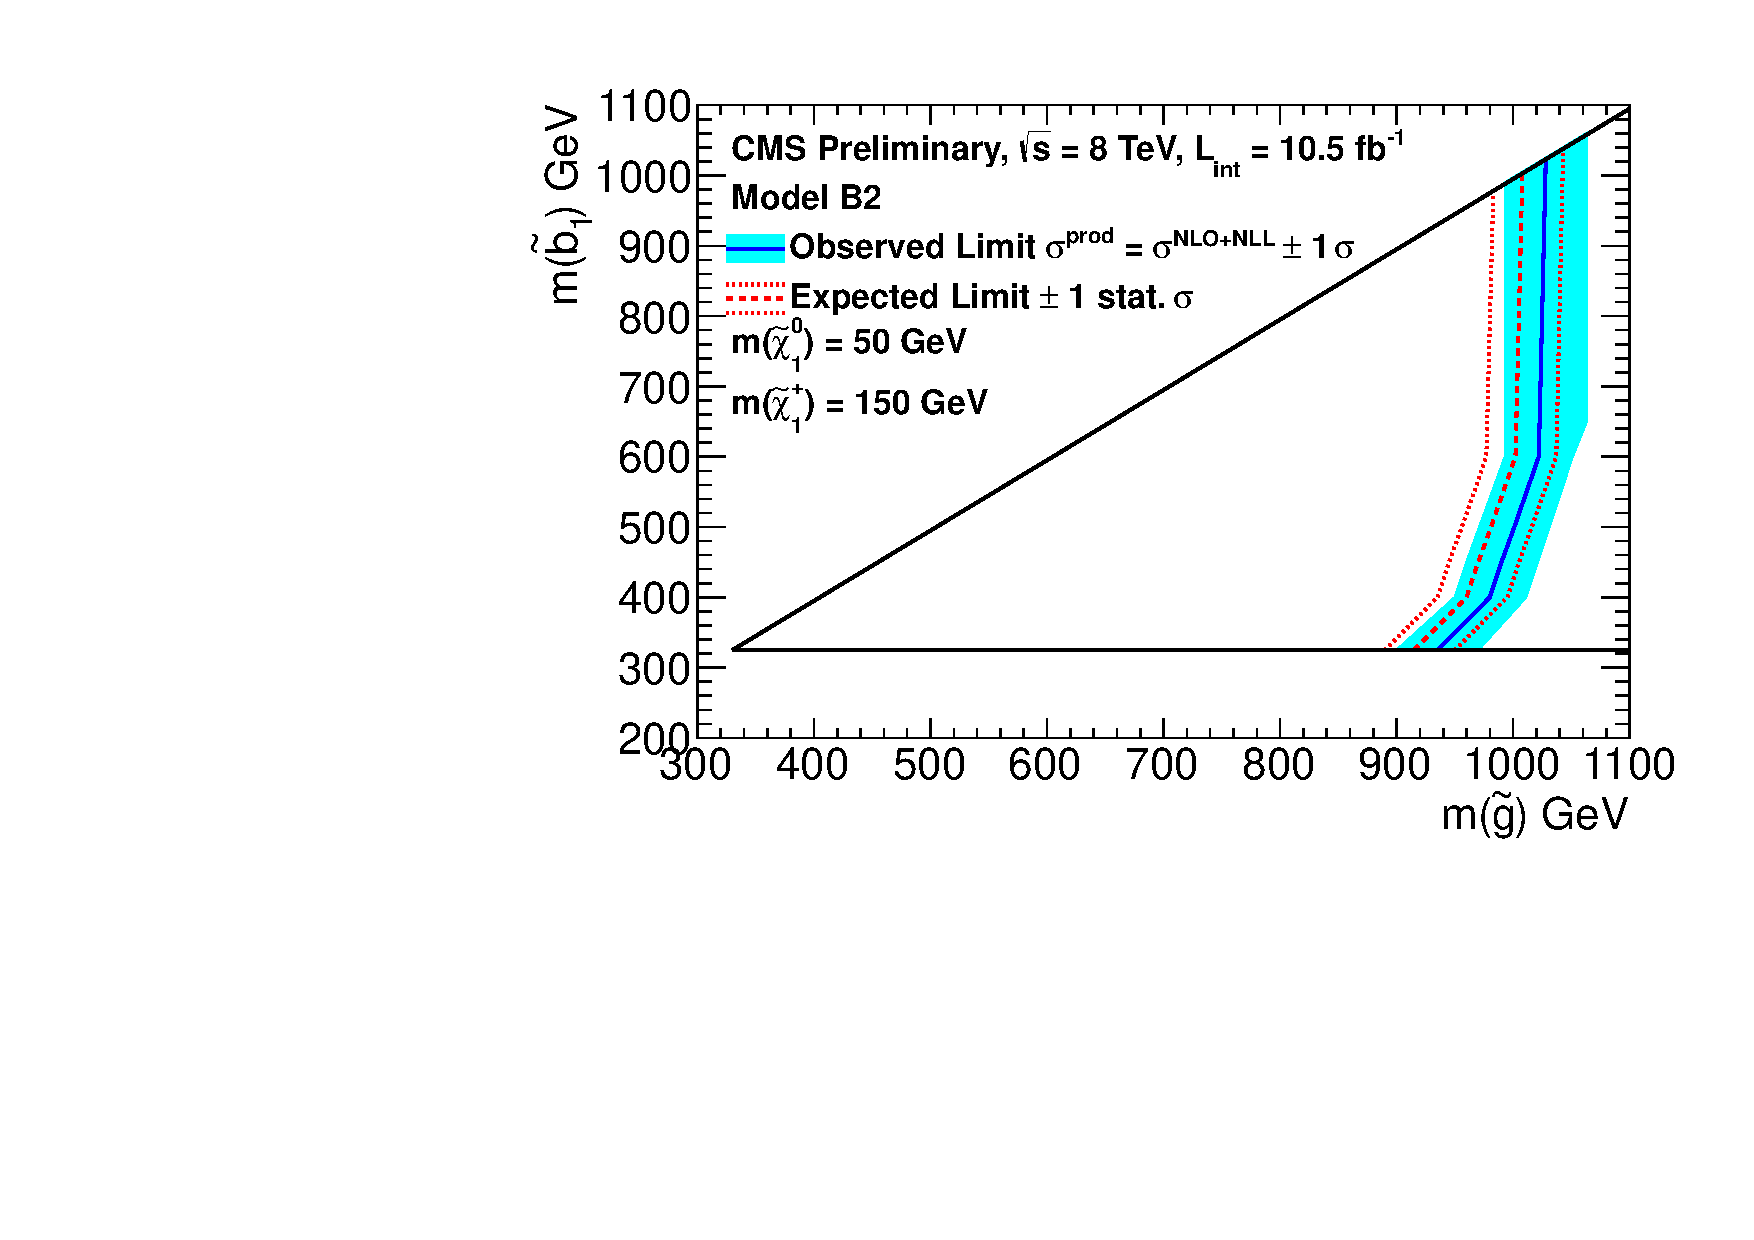
\includegraphics[width=0.45\textwidth]{HCPPlots/SS_B2.pdf} \\
\end{tabular}
\caption{
Interpretation of the results of the search in the same-sign dilepton final state in the model of gluino-mediated top squark production
of Fig.~\ref{fig:diagrams}b (left) and gluino-mediated bottom squark production of Fig.~\ref{fig:diagrams}d (right).
\label{fig:ss_interpretation}
}
%\end{center}
\end{figure*}


%\begin{table}
%\centering
%\caption{Please write your table caption here}
%\label{tab-1}       % Give a unique label
%% For LaTeX tables you can use
%\begin{tabular}{lll}
%\hline
%first & second & third  \\\hline
%number & number & number \\
%number & number & number \\\hline
%\end{tabular}
%% Or use
%\vspace*{5cm}  % with the correct table height
%\end{table}


\begin{table*}
\centering
  \caption{\label{tab:ss} Summary of the results of the search in the same-sign dilepton final state.
    Several signal regions (SR) are indicated, including the kinematic requirements, the prediction of the three background (BG) contributions,
    the total background, and the observed yield in data. The jet multiplicity requirement in the first row includes both b-tagged and untagged jets.}
  \tabcolsep 2.7pt
  \begin{scriptsize}
    \begin{tabular}{l|c|c|c|c|c|c|c|c|c}
\hline
\hline
& SR0 & SR1 & SR2 & SR3 & SR4 & SR5 & SR6 & SR7 & SR8 \\
      \hline
      No. of jets            & $\geq 2$               & $\geq 2$               & $\geq 2$               & $\geq 4$               & $\geq 4$               & $\geq 4$               & $\geq 4$               & $\geq 3$               & $\geq 4$       \\
      No. of btags           & $\geq 2$               & $\geq 2$               & $\geq 2$               & $\geq 2$               & $\geq 2$               & $\geq 2$               & $\geq 2$               & $\geq 3$               & $\geq 2$       \\
      Lepton charges         & $++/--$                & $++/--$                & $++$                   & $++/--$                & $++/--$                & $++/--$                & $++/--$                & $++/--$                & $++/--$        \\
      \met                 & $> 0$ GeV             & $> 30$ GeV            & $> 30$ GeV            & $> 120$ GeV           & $> 50$ GeV            & $> 50$ GeV            & $> 120$ GeV           & $> 50$ GeV            & $> 0$ GeV     \\
      $H_T$                  & $> 80$ GeV            & $> 80$ GeV            & $> 80$ GeV            & $> 200$ GeV           & $> 200$ GeV           & $> 320$ GeV           & $> 320$ GeV           & $> 200$ GeV           & $> 320$ GeV   \\
      \hline
      Charge-flip BG         & $3.35 \pm 0.67$ & $2.70 \pm 0.54$ & $1.35 \pm 0.27$ & $0.04 \pm 0.01$ & $0.21 \pm 0.05$ & $0.14 \pm 0.03$ & $0.04 \pm 0.01$ & $0.03 \pm 0.01$ & $0.21 \pm 0.05$\\
      Fake BG                & $24.77 \pm 12.62$ & $19.18 \pm 9.83$ & $9.59 \pm 5.02$ & $0.99 \pm 0.69$ & $4.51 \pm 2.85$ & $2.88 \pm 1.69$ & $0.67 \pm 0.48$ & $0.71 \pm 0.47$ & $4.39 \pm 2.64$  \\
      Rare SM BG             & $11.75 \pm 5.89$ & $10.46 \pm 5.25$ & $6.73 \pm 3.39$ & $1.18 \pm 0.67$ & $3.35 \pm 1.84$ & $2.66 \pm 1.47$ & $1.02 \pm 0.60$ & $0.44 \pm 0.39$ & $3.50 \pm 1.92$  \\
      \hline
      Total BG               & $39.87 \pm 13.94$ & $32.34 \pm 11.16$ & $17.67 \pm 6.06$ & $2.22 \pm 0.96$ & $8.07 \pm 3.39$ & $5.67 \pm 2.24$ & $1.73 \pm 0.77$ & $1.18 \pm 0.61$ & $8.11 \pm 3.26$  \\
      Event yield            & 43                & 38                & 14                & 1                & 10                & 7                & 1                & 1                & 9              \\
      \hline
%      $N_{{UL}}$ (13\% unc.) & 27.2   &26.0   &9.9    &3.6    &10.8   &8.6    &3.6    &3.7    &9.6 \\
%      $N_{{UL}}$ (20\% unc.) & 28.2   &27.2   &10.2   &3.6    &11.2   &8.9    &3.7    &3.8    &9.9 \\
%      $N_{{UL}}$ (30\% unc.) & 30.4   &29.6   &10.7   &3.8    &12.0   &9.6    &3.9    &4.0    &10.5 \\
      \hline
    \end{tabular}
  \end{scriptsize}
\end{table*}

\section{Search in the All-Hadronic Final State}
\label{sec:alphat}

\begin{figure*}[!ht]
\centering
%\begin{center}
\begin{tabular}{cc}
\subfloat[] {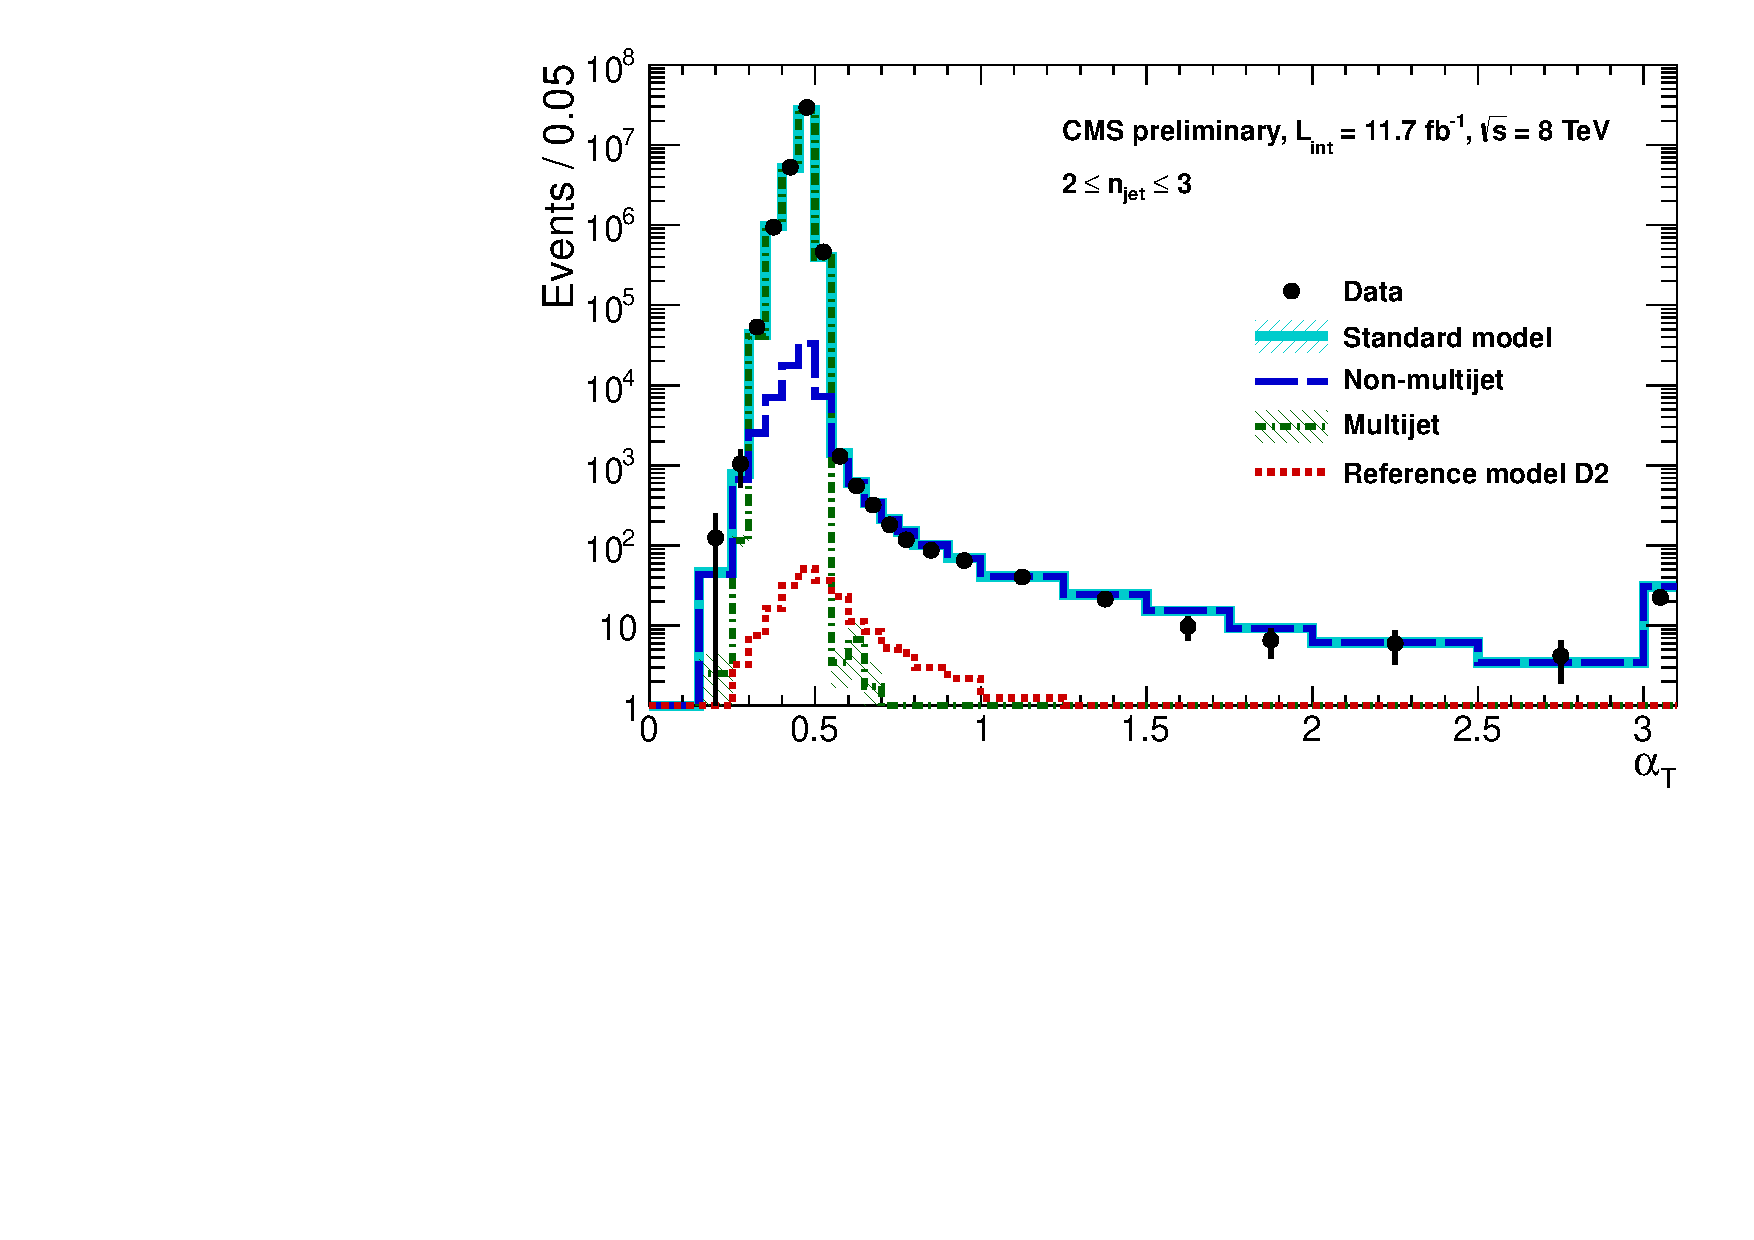
\includegraphics[width=0.45\textwidth]{HCPPlots/AlphaT_le3j_prelim.pdf}} &
\subfloat[] {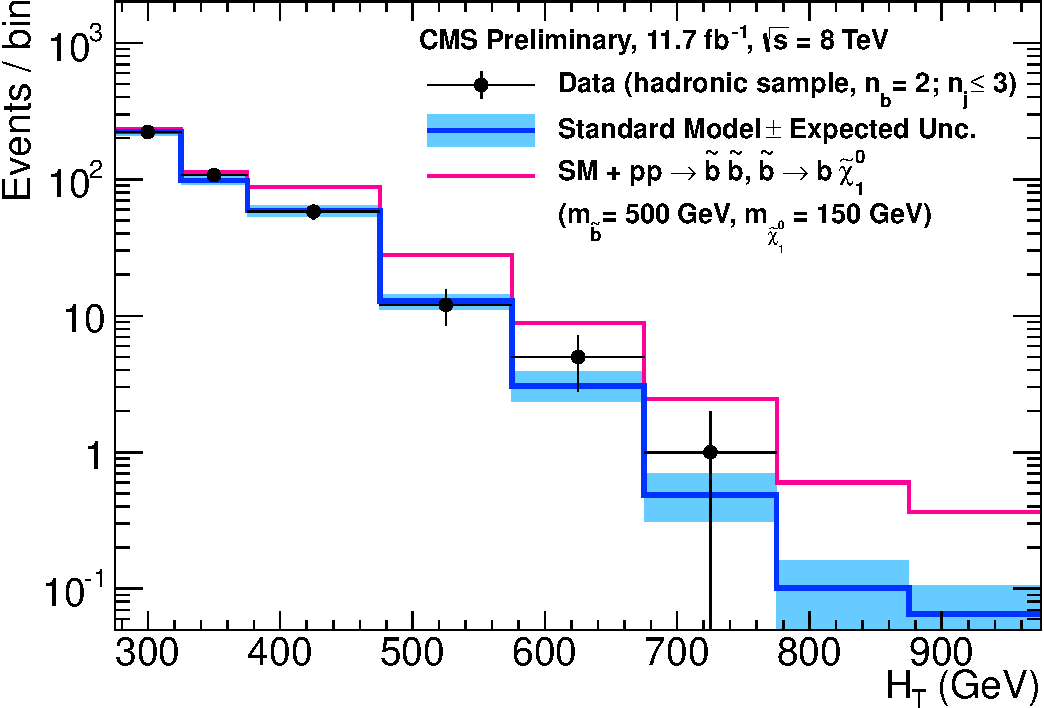
\includegraphics[width=0.4\textwidth]{HCPPlots/hadronic_2b_le3j_logy.pdf}} \\
\end{tabular}
\caption{
Distributions of \alphat\ (left) and $H_T$ (right) in data, compared to the SM background expectations.
An example signal scenario of bottom squark pair production with $\tilde{b}\to b\lsp$ is overlaid.
\label{fig:alphat}
}
%\end{center}
\end{figure*}

The production of bottom squark pairs, followed by the decay $\tilde{b}\to b\lsp$, leads to events with
two b-jets and \met. In this section we report the results from a search with 11.7 fb$^{-1}$ 
in the all-hadronic final state using the 
\alphat\ variable.%, discussed below, which discriminates between backgrounds with real and fake \met.

We count jets with \pt\ $>$ 50 GeV. The leading (highest \pt) jet is required to be in the tracker 
acceptance defined by $|\eta|<2.5$, and the leading two jets must satisfy \pt\ $>$ 100 GeV. Events with isolated 
electrons or muons with \pt\ $>$ 10 GeV are vetoed, in order to suppress backgrounds with neutrinos from the decays 
of W bosons. Events with an isolated photon with \pt\ $>$ 25 GeV are vetoed.
The remaining events are categorized based on the jet multiplicity, the number of b-tagged jets (using CSVM) and the event $H_T$, 
which is required to satisfy $H_T$ $>$ 275 GeV.

The background satisfying the above preselection is dominated by QCD multijet production with fake \met\ from mismeasurement effects. To suppress this background,
we require the events to have large $\alphat$. For dijet events this quantity is defined as $\alphat \equiv E_{T}^{j_2} / M_{T}$, where $E_{T}^{j_2}$ is the $E_T$
of the second leading jet and $M_T$ is the transverse mass of the dijet system. 
For events with perfectly measured jets, the reconstructed \pt\ values of the two jets are equal, leading to $\alphat=0.5$. 
%The key feature of the \alphat\ variable is that mismeasurement effects tend to decrease the value of \alphat, such that it is 
%extremely rare for events with fake \met\ to have \alphat\ much larger than 0.5. As shown in Fig.~\ref{fig:alphat}(a), 
%the \alphat\ distribution for the QCD multijet background falls off extremely rapidly near this endpoint value. 
The key feature of the \alphat\ variable is that mismeasurement effects tend to decrease the value of \alphat,
resulting in an endpoint at $\alpha_T\approx0.5$ for the QCD multijet background, which is evident in Fig.~\ref{fig:alphat}(a).
For events with three of more jets, an equivalent dijet 
system is formed by  clustering the jets into two pseudo-jets. In our search we strongly suppress the QCD multijet background with 
the requirement \alphat\ $>$ 0.55.

The background after the \alphat\ requirement is dominated by processes with genuine \met, including \ttljets\ and \wjets\ with a lepton and neutrino from W decay,
where the lepton is either not reconstructed or is a hadronically decaying $\tau$ lepton. 
These backgrounds are estimated using a $\mu+\rm{jets}$ data control sample.
The additional background from $\rm{Z}(\nu\nu)+\rm{jets}$ is estimated using two data control samples of $\rm{Z}(\ell\ell)+\rm{jets}$ and  $\gamma+\rm{jets}$ events. To estimate these backgrounds, the observed yields in the data control samples are extrapolated to the
signal region using translation factors derived from MC. The dominant systematic uncertainties in the background prediction stem from the uncertainties
in the MC translation factors, which are assessed by performing several closure tests in data. In these tests, the observed yields in one data control region
are used to predict the yields in another data control region.

Events are categorized based on the $H_T$, jet multiplicity, and b-tagged jet multiplicity. For the bottom squark scenario described above, the most sensitive
category is events with either two or three jets and exactly two b-tagged jets. The $H_T$ distribution for these events is indicated in Fig.~\ref{fig:alphat}(b),
which demonstrates good agreement between the data and the expected background. No evidence for an excess of events is observed.

The results are interpreted  using the model of bottom squark pair production with $\tilde{b}\to b\lsp$, in Fig.~\ref{fig:ss_interpretation}(b).
These results probe bottom squarks with masses up to approximately 600 GeV. Additional interpretations in models with gluino-mediated
top and bottom squark pair production are presented in Ref.~\cite{ref:alphat}.


\section{Summary}

This note presents a search for BSM physics in final states with leptonically-decaying Z bosons, jets, and \MET. 
Two strategies were pursued. The first is an inclusive approach which targets BSM scenarios with Z bosons produced
in the decays of strongly-interacting particles. The second is a targeted approach which focuses on BSM scenarios
where the Z bosons are produced in the decays of weakly-interacting particles. The main backgrounds are
estimated with data-driven techniques. Good agreement is observed between the data and the predicted backgrounds
over the full \MET\ range, for both searches. The results are interpreted in the context of a simplified SUSY
model where chargino-neutralino pairs decay to the \wzmet\ final state, and used to place constraints on the
masses of these particles.


%\section{Introduction}
%\label{intro}
%Your text comes here. Separate text sections with

%
% BibTeX or Biber users please use (the style is already called in the class, ensure that the "woc.bst" style is in your local directory)
% \bibliography{name or your bibliography database}
%
% Non-BibTeX users please use
%
\begin{thebibliography}{}
%
% and use \bibitem to create references.
%
%\bibitem{RefJ}
%% Format for Journal Reference
%Journal Author, Journal \textbf{Volume}, page numbers (year)
%% Format for books
%\bibitem{RefB}
%Book Author, \textit{Book title} (Publisher, place, year) page numbers
%% etc

\bibitem{ref:naturalsusy}
M. Papucci, J. T. Ruderman, and A. Weiler, arXiv:1110.6926 (2011).

\bibitem{ref:CMS}
CMS Collaboration, JINST \textbf{3}, S08004 (2008).

\bibitem{ref:stop}
CMS Collaboration, CMS-PAS-SUS-12-023 (2012).

\bibitem{ref:ss}
CMS Collaboration, arXiv:1212.6194 [hep-ex] (2012).

\bibitem{ref:alphat}
CMS Collaboration, CMS-PAS-SUS-12-028 (2012).

\bibitem{ref:btag}
CMS Collaboration, arXiv:1211.4462 [hep-ex] (2012).

\bibitem{ref:atlasstop}
ATLAS Collaboration, Phys. Rev. Lett. \textbf{109}, 211803 (2012).

\bibitem{ref:ss_inclusive}
CMS Collaboration, Phys. Rev. Lett. \textbf{109}, 071803 (2012).

\end{thebibliography}

\end{document}

% end of file template.tex

